\documentclass{article}

\usepackage{graphicx}
\usepackage[margin=2cm,twocolumn,columnsep=5mm]{geometry}
\usepackage[tableposition=top]{caption}
\captionsetup{font=small}

\usepackage{hyperref}
\usepackage[dvipsnames]{xcolor}
\hypersetup{colorlinks=true,urlcolor=MidnightBlue,citecolor=Blue,linkcolor=Blue}

\usepackage[backend=biber,citestyle=numeric]{biblatex}
\addbibresource{/home/nate/Dropbox/nates-biblio-DB.bib}

\usepackage{setspace}
\setstretch{1.25}

\title{Toronto Bike Map \\ Project Prospectus}
\author{Nate Wessel, PhD \\ \small \href{mailto:bike756@gmail.com}{bike756@gmail.com}}

\begin{document}
	\maketitle
	%Our streets and roads, as they now exist, were built for cars. Cyclists in North America, though growing in numbers, have had almost none of the slow, fluvial influence of a full century of widespread automotivity. Yet in the eddies and on the margins thin tendrils of cycling infrastructure have crept their way into an increasingly fractured rock. The scene is still chaotic, the way forward unclear. 
	
	\section*{Background}
		In the winter of 2014 I began a project to ``rethink the urban bike map.'' 
		I was living in Cincinnati, Ohio and I had grown frustrated with the maps I could find to help me navigate by bike. One genre of maps in particular, produced locally by our MPO, listed streets which were {\color{ForestGreen}good} or {\color{red}bad} for cycling. As an independent-minded person, this struck me as at least a little condescending, especially as I knew the human source of the these judgments was a single and not uniquely representative cyclist.
		Another genre, generally available online, overlaid bike-specific infrastructure on a standard street map. This being not the Netherlands however, that infrastructure was hopelessly fragmented while the map that remained uncovered was essentially a map for cars.\footnote{This seems to be the dominant paradigm in Toronto. E.g. \href{https://www.toronto.ca/services-payments/streets-parking-transportation/cycling-in-toronto/cycling-google-map/}{https://www.toronto.ca/services-payments/streets-parking-transportation/cycling-in-toronto/cycling-google-map/}}
	
		I decided I would publish my own map, something I had done a few years before after our local transit agency had failed to create a decent system map on their own.
		My idea was that the new bike map should be thoroughly \textit{objective} and that it also needed to show much more than just the disjunct and miscellaneous bike lanes and cycletracks of other maps. I classified every street according to its width and speed limit, highlighting those with restricted auto access and emphasizing bike lanes where they existed. Cincinnati has quite a few cul-de-sacs and one of the more innovative ideas I had was to detect these using an algorithm borrowed from graph theory so that these could be de-emphasized relative to other streets.\footnote{
			Tarjan's algorithm for the detection of strongly connected subcomponents. Any edge not belonging to the main strongly connected component was rendered partly transparent.
		} Dead-end signs have always bothered me - a dead end for a car may not be a dead-end for a bike or a pedestrian as indeed it often isn't. Access restrictions on each way were used to define dead-ends \textit{for cyclists}. 
		This cycling-specific measure of network connectivity ended up rather dramatically improving the readability of the map. 
		By spring of 2015, I had printed and distributed the map (9,000 paper copies and online) with the help of a local foundation and several generous sponsors. The project as well as the history and thought behind it have been thoroughly documented in an article in Cartographic Perspectives which is freely available online.\footnote{
			\fullcite{Wessel2015}
		}
	
	\section*{A Smarter Approach}
	
		As I used my new map for actual navigation I began to wonder if there weren't better, more elegant ways of defining connectivity from a cyclist's perspective. By mapping road width onto the width of lines on the map (See Figure \ref{fig:legend}), I had introduced a somewhat car-oriented perspective; bigger streets with more lanes for cars were generally bigger and bolder on my map, regardless of their utility for cyclists. 
		
		\begin{figure}[h!]
			\centering
			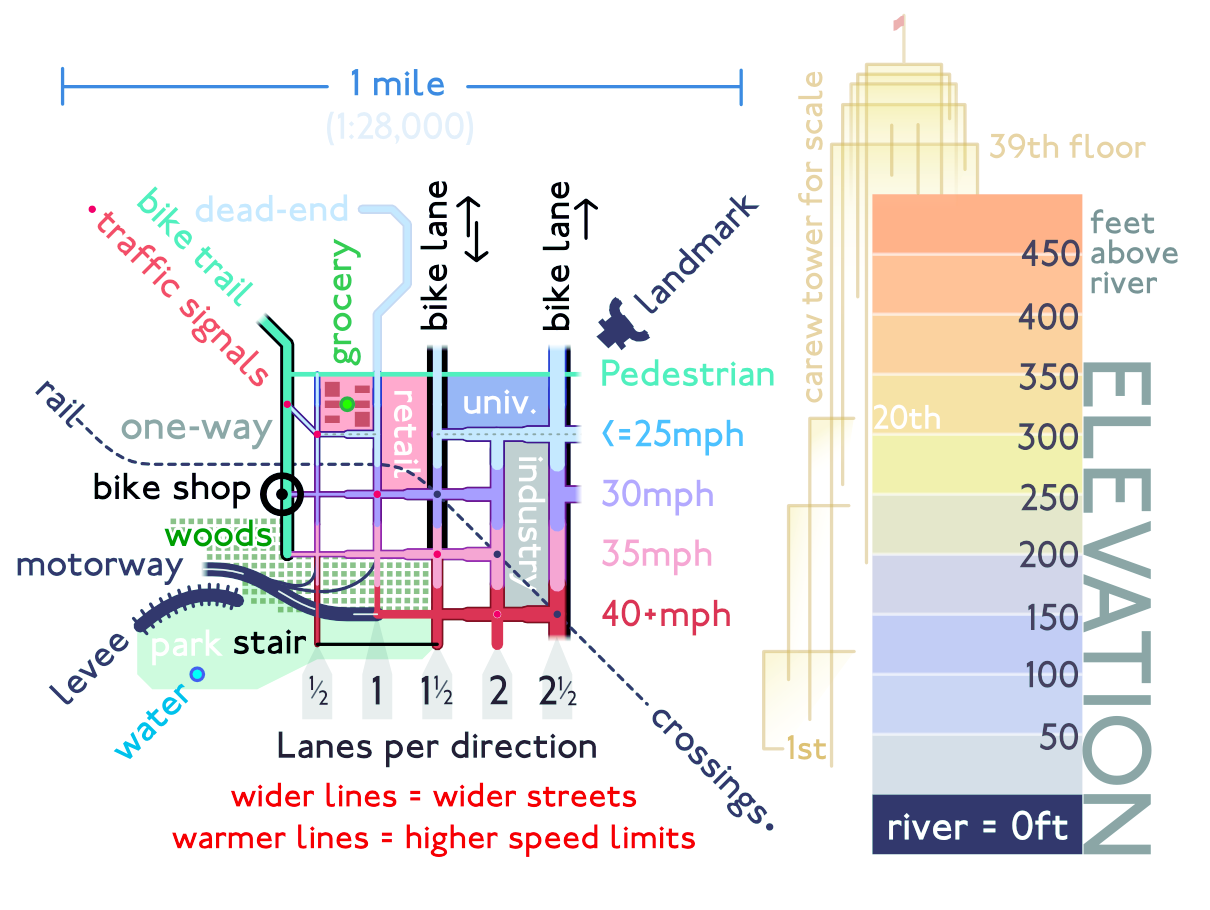
\includegraphics[width=0.4\textwidth]{legend}
			\caption{From the legend of the Cincinnati Bike Map.}
			\label{fig:legend}
		\end{figure}
		
		I was using data from OpenStreetMap which allows every edge and node in the street network to have mode-specific access restrictions. Indeed, several advanced trip-planning applications exist specifically to use OpenStreetMap data to help cyclists plan trips according to their preferences and limitations. I eventually discovered that I could use one of these trip planners to readily approximate a measure of \textit{betweenness centrality}. This concept, borrowed again from graph theory, essentially measures the importance of links in a network by counting the number of least-cost paths across that network in which they play a part. 
		By using a realistic trip-planner to simulate a large set of bicycle trips across the street network I could thus estimate the relative importance of every street segment from a cyclist's perspective.\footnote{
			This is very similar conceptually to the problem of traffic assignment in transport modelling, where my measure of ``importance'' is comparable to an estimate of traffic volume. Congestion however need not be taken into account and the pattern of travel demand need not be realistic. 
		}
		This approach would implicitly mute dead-ending streets and also highlight streets which played an important part in the cycling network, regardless of their particular characteristics or the (non)presence of bike infrastructure. 
		
		Thus for example if we have a street with a long, useful bike lane, but that lane has gaps and discontinuities, we may see that the segments connecting the portions with bike lanes are just as important in the street hierarchy as those segments with their own bike lanes. Presenting a continuous visual hierarchy to cyclists should make the network easier to navigate. This is illustrated in Figure \ref{fig:spanned-gap} where the algorithm picks up an important connection between the bike lanes on Lansdowne Avenue and The Queensway. 
		\begin{figure}[h!]
			\centering
			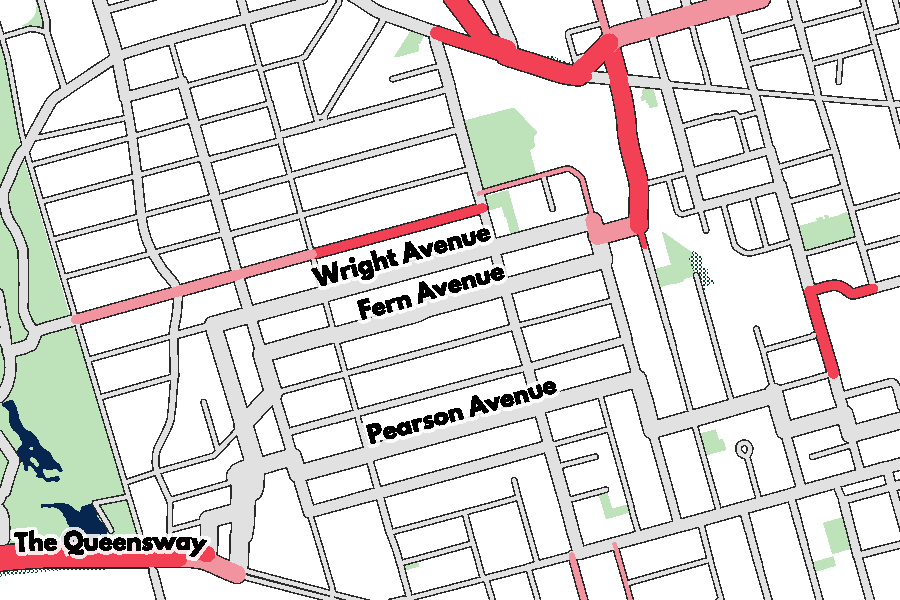
\includegraphics[width=0.45\textwidth]{spanned-gap}
			\caption{Wright and Fern Avenues are shown to be important in connecting trips using the bike lanes on Lansdowne Avenue and The Queensway, despite the presence of a bike lane one block north on Fermanagh.}
			\label{fig:spanned-gap}
		\end{figure}
	
		\section*{Reframing the city}
		Our culture is often radically oriented toward automobility, and this  auto-oriented perspective is even encoded into the geospatial network data used to produce maps advocating for cyclists. Streets are universally graded into a hierarchy based on their suitability for auto travel, and these visual hierarchies, relayed to us in almost every map we see, form a familiar picture. 
		
		Preliminary analysis shows that the resulting visual hierarchy is substantially different from that shown on other maps of the city which are primarily oriented around auto-travel.\footnote{
			http://natewessel.com/2017/mapping-modal-hierarchy/
		} 
	
\end{document}